\documentclass[a4paper]{scrartcl}

%\usepackage{showframe}
\usepackage[margin=2cm,footskip=.7cm]{geometry}
\usepackage{enumitem}
% \usepackage{fourier}
\usepackage{xcolor}
% \usepackage{abkuerzungen}
\usepackage{hyperref}
\usepackage{amsmath}
\usepackage{../../ISASmacros/isasmathmacros}

\usepackage{pdfpages}


\newcommand{\sA}{\ensuremath{\mathsf{A}}}
\newcommand{\sAB}{\ensuremath{\mathsf{AB}}}
\newcommand{\sB}{\ensuremath{\mathsf{B}}}
\newcommand{\sBA}{\ensuremath{\mathsf{BA}}}
\newcommand{\sC}{\ensuremath{\mathsf{C}}}

\newcommand{\cest}{\ensuremath{\cvec{\gamma}}}
\newcommand{\cerest}{\ensuremath{\ervec{\gamma}}}
\newcommand{\cmat}{\ensuremath{\mat{\Gamma}}}
\newcommand{\tmat}{\ensuremath{\widetilde{\mat{\Gamma}}}}

\newcommand{\gainA}{\ensuremath{\mat{K}}}
\newcommand{\gainB}{\ensuremath{\mat{L}}}

% \newcommand{\fus}{\ensuremath{\op{fus}}}

% \newcommand{\CI}{\op{CI}\xspace}
% \newcommand{\EI}{\op{EI}\xspace}
% \newcommand{\ICI}{\op{ICI}\xspace}
% \newcommand{\BC}{\op{B\!/\!C}\xspace}
% \newcommand{\ind}{\op{s}\xspace}
\newcommand{\ind}{\op{in}\xspace}
\newcommand{\opt}{\cmat}


\newcommand{\excmat}{\ensuremath{\mat{\Gamma}'}}
\newcommand{\excest}{\ensuremath{\cest'}}
% \newcommand{\exoptmat}{\ensuremath{\mat{C}_{\excmat}}}
\newcommand{\exoptmat}{\ensuremath{\mat{C}'_\EI}}

%\RequirePackage[mathscr]{euscript}
%\RequirePackage{bbding}
%\RequirePackage{scalefnt}
%\RequirePackage{mathtools}
% This was enabled but makes the text look ugly
%\RequirePackage[T1]{fontenc}


%%% COLOR DEFINITIONS

% KIT Colors
\definecolor{kitgreenex}{RGB}{0,152,131}
\definecolor{kitblueex}{RGB}{52,115,186}
\definecolor{kitmaygreen}{RGB}{119,184,38}
\definecolor{kityellow}{RGB}{255,228,0}
\definecolor{kitorange}{RGB}{247,154,0}
\definecolor{kitbrown}{RGB}{182,130,28}
\definecolor{kitred}{RGB}{187,25,23}
\definecolor{kitpurple}{RGB}{190,0,126}
\definecolor{kitcyanblue}{RGB}{0,167,227}
% Own Definitions
\definecolor{grey}{RGB}{150,150,150}


\definecolor{nblue}{RGB}{54,95,145}

%%% FONTS
%\setkomafont{pageheadfoot}{\small\color{darkgray}}
%\setkomafont{pagefoot}{\normalfont\color{darkgray}}
%\setkomafont{pagenumber}{\color{darkgray}}
%\setkomafont{captionlabel}{\small\bfseries\color{darkgray}}
\setkomafont{disposition}{\bfseries}
\setkomafont{section}{\normalfont\large\bfseries}
\setkomafont{subsection}{\normalfont\bfseries}
\setkomafont{author}{\normalfont}
\setkomafont{date}{\normalfont}


%%% PARAGRAPH LAYOUT
\setlength{\parindent}{0mm}
\setlength{\parskip}{6pt}


%%% REBUTTAL COMMANDS
\newenvironment{rebuttal}{\begin{enumerate}[label={\color{grey}\thesection.\arabic{enumi}},leftmargin=0pt,ref=\thesection.\arabic{enumi}]}{\end{enumerate}}
\newcommand{\reviewtext}[1]{{\color{nblue} #1}}
\newcommand{\papertext}[1]{\emph{``#1''}}

%%% HYPERREF SETUP
\hypersetup{
        colorlinks = true,
        linkcolor = kitgreenex
}

%%%%%%%%%%%%%%%%%%%%%%%%%%%%%%%%%%%%%%%%%%%%%%%%%%%%%%%%%%%%%%%%%%%%%%%%

\title{\boldmath Privacy-Preserving Localization Using Private Linear-Combination Aggregation}
\subtitle{Response to Reviewers' Comments - Submission IEEE-TAC 20-2108}
\author{Marko Ristic\and Benjamin Noack\and Uwe D. Hanebeck}

%       .d8888b.  888                     888
%      d88P  Y88b 888                     888
%      Y88b.      888                     888
%       "Y888b.   888888  8888b.  888d888 888888
%          "Y88b. 888        "88b 888P"   888
%            "888 888    .d888888 888     888
%      Y88b  d88P Y88b.  888  888 888     Y88b.
%       "Y8888P"   "Y888 "Y888888 888      "Y888

\begin{document}

\maketitle

Dear Dr. Zhiwei Gao,\\
Dear Reviewers,

We would like to thank you all for your thorough and helpful reviews. In this letter, we will describe how editor and reviewer comments, questions and suggestions have been addressed. Throughout this response, reviewers' comments are in \reviewtext{blue}. 

Sincerely,\\
Marko Ristic, Benjamin Noack, and Uwe D. Hanebeck

%      8888888888     888 d8b 888
%      888            888 Y8P 888
%      888            888     888
%      8888888    .d88888 888 888888 .d88b.  888d888
%      888       d88" 888 888 888   d88""88b 888P"
%      888       888  888 888 888   888  888 888
%      888       Y88b 888 888 Y88b. Y88..88P 888
%      8888888888 "Y88888 888  "Y888 "Y88P"  888



\section*{Response to the Editor's Report}
\def\thesection{E}
\begin{rebuttal} %\setcounter{enumi}{-1}
\item \reviewtext{Based on the reviews, it is our decision that the paper cannot be accepted for publication in the Transactions in its present form.

The reviewers feel the paper interesting, which many include publishable materials. On the other hand, the reviewers feel the paper should be reorganized by shortening the length (e.g. introduction etc.), and highlight the novelty and contribution. Also the relevance of the paper to the journal should be clarified.}

Thank you for the response. We have undertaken a large overhaul of the manuscript in order to accomodate for the suggested changes of the reviewers. The work has been shortened by four pages, the introduction shortened to a single page and the novelty of our method clearly stated within it. We state the estimation problem tackled, namely, a modified EKF estimator for range-only sensor localisation with specific security requirements, and its benefits over existing and comparable approaches. We believe that the more clarified contribution and novelty also better justifies the relevance of the paper to the TAC journal.

\item \reviewtext{We encourage you to examine carefully the comments of the enclosed reviews and to consider making a major revision of the paper, which can be resubmitted as a Technical Note, to the Transactions on Automatic Control.  If you do submit a revised version of the paper as a Technical Note, you should take care that the paper is reduced to no
more than 8 double-column pages using IEEE template.

In your letter of transmittal, you should include a detailed "author's response" document describing the changes in the paper and you should refer to the present paper number.

Please login, click on the "Author" link at the bottom of your access page, and upload your technical note under the SAME reference number. A new reference number will be assigned to your revised paper.}

After a large revision of our manuscript, including the suggested additions and modifications from the reviewers, we have rearranged and greatly shortened the work (in particular the introduction and cryptography sections, but all sections have been partially modified to be clearer). Due to the novelty of the tackled problem and the cryptographically backed solution, the manuscript, albeit four pages shorter, is still too long for submission as a Technical Note, and we would like to resubmit the work as a full paper again. We hope that this decision is made clearer from the newly revised and rearranged manuscript. Below, we have detailed how each of the reviewer comments have been taken into account when revising the work.

\end{rebuttal}

%      8888888b.                         d888
%      888   Y88b                       d8888
%      888    888                         888
%      888   d88P .d88b.  888  888        888
%      8888888P" d8P  Y8b 888  888        888
%      888 T88b  88888888 Y88  88P        888
%      888  T88b Y8b.      Y8bd8P         888
%      888   T88b "Y8888    Y88P        8888888



\section*{Response to the Comments of Reviewer 1 (222511)}
\def\thesection{R1}
\begin{rebuttal}
\item \reviewtext{This paper concerns the localization problem under privacy constraints. Cryptographic schemes have been devised by the authors to achieve some privacy requirements. The contribution is significant enough and the paper is well written but hard to understand for a usual reader of IEEE TAC due to sections with cryptographic background.}

We thank the reviwer for their comment on our contribution and are sorry that the work was not made easier to understand. We have rearranged the paper to make both the problem tackled and the solution presented easier to follow and more concise. Additionally we have greatly reduced the amount of cryptographic background presented, and hope that these changes make the work much easier to follow for the usual target audience of IEEE TAC.

\item \reviewtext{As a TAC paper, performance analysis in terms of estimation accuracy was expected but is actually missing.}

We regret that the method of analysis for our approach was not made clearer. As the proposed method we present is ineherently a modified EKF, we directly compare the estimation accuracy of our method to the industry standrd EKF (EIF reformulation in our case). To make this clearer, we have rewritten the results section to portray this evaluation better, and changed the results figure to be far more legible. Direct comparisons beween the EIF and our method are now made for each simluation considered, and the estimation error (accuracy of the filters) can be seen much more clearly. We hope this makes the evaulation of the presented method easier to understand.

\item \reviewtext{This reviewer wonders if IEEE TAC is well adapted for an efficient exposition of the authors' findings.}

We agree that the state of the initial submission was not as well suited to the TAC journal as could be desired and thank the reviewer for pointing this out. For the resubmission, we have greatly reduced the cryptographic components of the work and stated our contribution and its novelty more clearly to clarify the suitability of the proposed estimation method to the TAC journal. We will additionally consider some of the heavier cryptographic computations presented for an alternative submission elsewhere.

\item \reviewtext{In the framework of a Control theory paper, cryptographic notions would be kept as minimum as possible in the main body of the paper or moved to Appendices.}

As above, we regret that the quantity of presented cryptographic content was so poorly suited to the context of TAC and have greatly modified the work to make it a better fit. Much of the cryptographic discussion has been removed and the remaining, necessary but dense, novel notions have been put in the appendix. We hope this makes the work better suited in the context of TAC.

\end{rebuttal}

%      8888888b.                         .d8888b.
%      888   Y88b                       d88P  Y88b
%      888    888                              888
%      888   d88P .d88b.  888  888           .d88P
%      8888888P" d8P  Y8b 888  888       .od888P"
%      888 T88b  88888888 Y88  88P      d88P"
%      888  T88b Y8b.      Y8bd8P       888"
%      888   T88b "Y8888    Y88P        888888888



\section*{Response to the Comments of Reviewer 2 (222527)}
\def\thesection{R2}
\begin{rebuttal}
\item \reviewtext{This paper deals with a suitable notion of linear-combination aggregation encryption and provides a cryptographically secure instance applied to a filter with range-sensor measurements. This approach keeps navigator location, sensor's location and sensors' measurements private during navigation.

The proposed approach is interesting and the results are technically sound. The literature review is OK. But the organization of paper and its length make its reading difficult.}

Our response.

\item \reviewtext{The reviewer encourages the authors to reorganize the article by greatly shortening it and to highlight the novelty.}

Our response.

\item \reviewtext{Some additional comments are given below:

-Introduction (2 pages) is too long and does not focus on the main ideas of the paper. There are too many reminders of classical notions.}

Our response.

\item \reviewtext{-Equation (3): i from 1 to n must be added.}

Our response.

\item \reviewtext{-The actual computation steps are in fact scattered all over the paper, in several sections.  In the current version, the reader has to collect all the scattered pieces to come out with the approach. I would therefore, strongly recommend the authors to summarize all the steps of the approach gathered by the end of the paper, to help the reader directly use and implement the algorithm.}

Our response.

\item \reviewtext{-Page 10, Equation (36), Right part of Equation: d is from 0 to D}

Our response.

\item \reviewtext{-Inequality (50) must be clarified,}

Our response.

\item \reviewtext{-Algorithm 1, steps 2/3/4, it is F\_\{k-1\},}

Our response.

\item \reviewtext{-Section VIII-some explanations on the process model must be added. Figure 6 is too small; it is difficult to distinguish the different lines.}

Our response.

\end{rebuttal}

%      8888888b.                         .d8888b.
%      888   Y88b                       d88P  Y88b
%      888    888                            .d88P
%      888   d88P .d88b.  888  888          8888"
%      8888888P" d8P  Y8b 888  888           "Y8b.
%      888 T88b  88888888 Y88  88P      888    888
%      888  T88b Y8b.      Y8bd8P       Y88b  d88P
%      888   T88b "Y8888    Y88P         "Y8888P"



\section*{Response to the Comments of Reviewer 3 (229727)}
\def\thesection{R3}
\begin{rebuttal}
\item \reviewtext{This paper presented a theoretical framework for privacy-preserving localisation combining the encryption scheme and filtering. In particular, the private linear-combination aggregation has been adopted in the presented framework. Basically, the contribution of the paper is clearly indicated with an interesting and important topic. However, some technical problems need to be further clarified. Therefore, a major revision is necessary in my opinion.}

Our response.

\item \reviewtext{1) Is any filtering method can be integrated into the presented framework? If so, can we replace the method via numerical approach such as particle filter.}

Our response.

\item \reviewtext{2) How does the linear combination reflect the dynamics of the investigated system in Eq.(2)?}

Our response.

\item \reviewtext{3) Why is the noise of the system Gaussian? In Eq.(2), function f() is known then what is the physical meaning of the Gaussian process noise?}

Our response.

\item \reviewtext{4) In the paper, the noise is depended on covariance matrix \$Q\$ which is also particularly used in Algroithm 1, however, in practice, Q is unmeasurable and unknown. How to estimate the value of Q in terms of performance guarantee.}

Our response.

\item \reviewtext{5) The experimental results are limited. The comparison is essential to validate the performance of the presented algorithm. What about using the existing filtering method to demonstrate the various encryption scheme?}

Our response.

\item \reviewtext{6) There are some typos in the manuscript please correct them, for example, page 1 Notation, '\$\textbackslash left\textbackslash\textbar\textbackslash underline a\textbackslash right\textbackslash\textbar\$ the vector norm' should be '\$\textbackslash left\textbackslash\textbar\textbackslash underline a\textbackslash right\textbackslash\textbar\$ is the vector norm' etc.}

Our response.

\end{rebuttal}

% 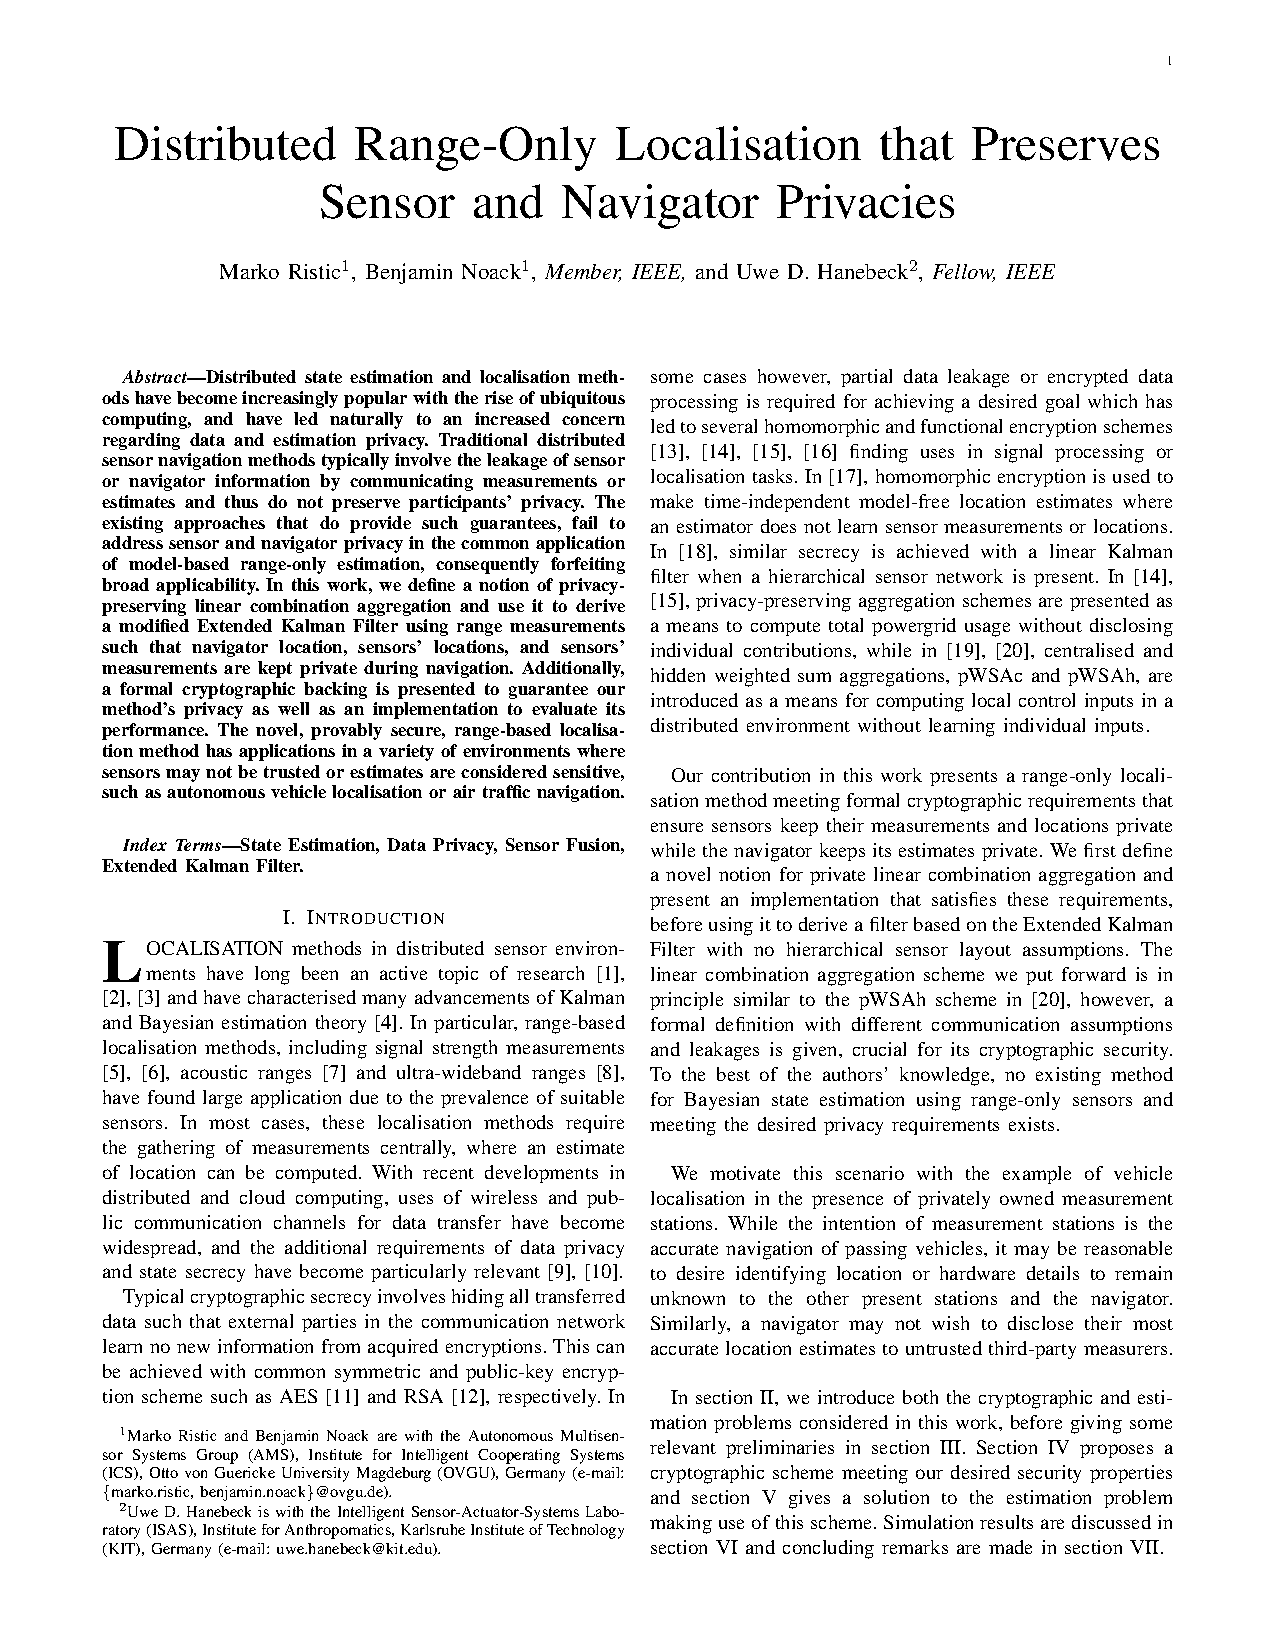
\includepdf[pages=-]{diff}

\end{document}